\chapter{Automate de Séquences}
\label{chap-sequence-automaton}
\index{Automate de Séquences}

La construction de grammaires locales peut être un long processus durant lequel le linguiste répète
de nombreuses fois les mêmes opérations. La finalité du programme \verb+Seq2Grf+ est de produire
rapidement et automatiquement des grammaires locales.


\bigskip
\noindent
Ce programme peut être utilisé en ligne de commande ou en cliquant sur "Construct Sequences
Automaton" dans le menu "Text". L'utilisation de la commande \verb+Seq2Grf+ est décrite à la
section~\ref{Seq2Grf}.

\bigskip
\noindent Pour un document donné (\verb+TEILite+ ou des fichiers au format \verb+txt+ ou \verb+SNT+
quand ils sont prétraités pour cette tâche avec des marqueurs \verb+{STOP}+) ce programme
construit un
unique automate qui reconnaît toutes les séquences contenues dans le document.

\bigskip
\noindent On doit porter une attention particulière à la construction de la liste de séquences qui
doivent être reconnues par le graphe.

\bigskip
\noindent Ce chapitre présente les formats de fichiers supportés par le programme \verb+Seq2Grf+, la
construction de l'automate de séquences et l'utilisation de jokers.
\bigskip


\section{Corpus de séquences}
\index{Corpus de séquences}
Nous appelons \textit{corpus de séquences}\index{Corpus de séquences} ou \textit{corpus qualifié}
\index{Corpus qualifié} une liste de séquences d'un ou plusieurs mots que l'on veut reconnaître par
une grammaire locale représentée par un seul graphe.
\bigskip

Le corpus de séquences est stocké dans un seul fichier qui peut avoir l'un des formats suivants :
\begin{itemize}
\item fichiers texte brut, dans lequel les séquences sont délimitées par des fins de lignes
\item fichiers \verb+SNT+ déjà prétraités par ce menu : les séquences sont délimitées
		par \verb+{STOP}+
\item fichiers \verb+TEILite+ dont les séquences sont délimitées par un tag \verb+xml+ de la
		forme :
%ne pas enlever le saut de ligne suivant

		\verb+<seg type="sequence">example</seg>}+
\end{itemize}
\pagebreak 
\indent Puisque le corpus contient des séquences spécifiques, il doit être fait à la main.
Cela signifie que vous devez soit écrire toutes les séquences dans un fichier texte brut et les
séparer par une fin de ligne (figure~\ref{fig8-1CorpusTxt}), soit insérer la balise \verb+XML+
spécifique dans un document existant \verb+TEILite+ (figure~\ref{fig8-3CorpusTEI}). Le prétraitement
des documents \verb+TXT+ ou \verb+XML+ génère un fichier \verb+SNT+ qui est utilisé pour la
construction de l'automate de séquences (figure~\ref{fig8-2CorpusSNT}). Ce fichier peut être utilisé
comme une entrée. Le graphe produit ne reconnaîtra que les séquences qui sont correctement
délimitées. La production de grammaires locales est automatique uniquement à partir d'un corpus de
séquences bien définies. Si vous disposez d'un tel corpus, alors le gain de temps est considérable.

\begin{figure}[h!]
	\begin{minipage}[h!]{0.5\linewidth}
		\centering
		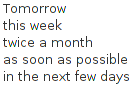
\includegraphics[scale=0.6]{resources/img/fig8-1tomorrow.png}	
		\caption{TXT\label{fig8-1CorpusTxt}}
		\label{fig7-TXT}
	\end{minipage}
	\hspace{0.1cm}
	\begin{minipage}[h!]{0.5\linewidth}
		\centering
		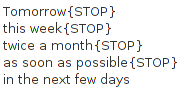
\includegraphics[scale=0.6]{resources/img/fig8-2tomorrowSNT.png}
		\caption{SNT\label{fig8-2CorpusSNT}}
	\end{minipage}
	\hspace{0.1cm}
\end{figure}
\begin{figure}[h!]
	\begin{minipage}[h!]{\linewidth}
		\centering
			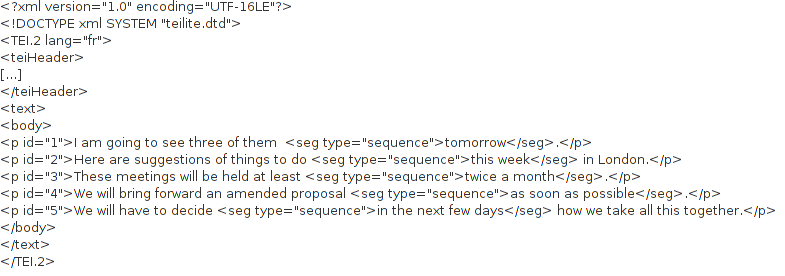
\includegraphics[width=14cm]{resources/img/fig8-3tomorrowTEI.png}
			\caption{TEILite\label{fig8-3CorpusTEI}}
	\end{minipage}
\end{figure}

%%%%%%%%%%%%%%%%%%%%%%%%%%%%%%%%%%%%%%%%%%%%%%%%%%%%%%%%%%%%%%%%%%%

\section{Utilisation}
Pour créer un automate de séquences, cliquez sur "Séquence Construct Automate" dans le menu "Text".
Vous verrez alors apparaître la fenêtre de la figure~\ref{fig8-4Menu1}.

Cette fenêtre vous permet de définir les paramètres pour produire un automate séquence.
Vous devez suivre ces trois étapes :
\begin{itemize}
\item choisissez le corpus séquences : celui-ci peut être un fichier dont le format est l'un des trois formats décrits dans la section précédente. Le format de fichier est automatiquement détecté en fonction de l'extension de fichier.

\item définissez les options spécifiques :
"Apply the beautifying algorithm" placera chaque boîte de manière à ce que le graphe résultant soit
le plus petit et le plus facile à lire que possible.
"Exact case matching" mettra les tokens littéraux entre accolades dans le graphe afin que ceui-ci ne
reconnaisse pas des tokens avec les mêmes lettres mais avec des différences de casse.

Vous pouvez définir des options supplémentaires pour produire un graphe qui permet une
reconnaissance approximative : vous pouvez fixer le nombre de jokers à utiliser pour produire de
nouvelles séquences dérivées des séquences du corpus original, et choisir le joker approprié. Tous les détails sur l'utilisation des jokers se trouvent dans la section
\ref{approximation}

\item choisissez le répertoire où le graphe sera enregistré.
\end{itemize}
\medskip
\begin{figure}[h!]
	\begin{minipage}[h!]{0.5\linewidth}	
		\centering
			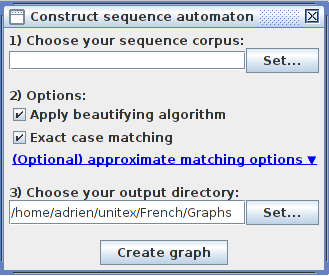
\includegraphics[width=8cm]{resources/img/fig8-4Menu1.png}
			\caption{Menu automate de séquences\label{fig8-4Menu1}}
	\end{minipage}	
	\hspace{0.3cm}
	\begin{minipage}[h!]{0.5\linewidth}	
		\centering
			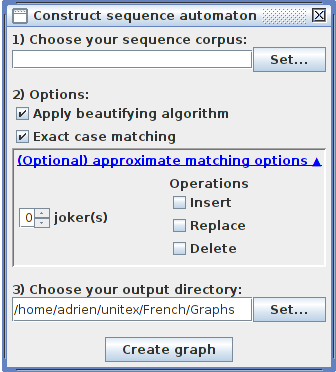
\includegraphics[width=8cm]{resources/img/fig8-4Menu2.png}
			\caption{Menu options de l'automate de séquences\label{fig8-4Menu2}}
	\end{minipage}
\end{figure}

\bigskip
\noindent Vous pouvez voir figures~\ref{fig8-5GRFnoBeautify} et ~\ref{fig8-6GRFBeautify} les graphes
sans jokers produits avec ou sans "beautify".


\begin{figure}[h!]
	\begin{minipage}[h!]{0.5\linewidth}
		\centering
		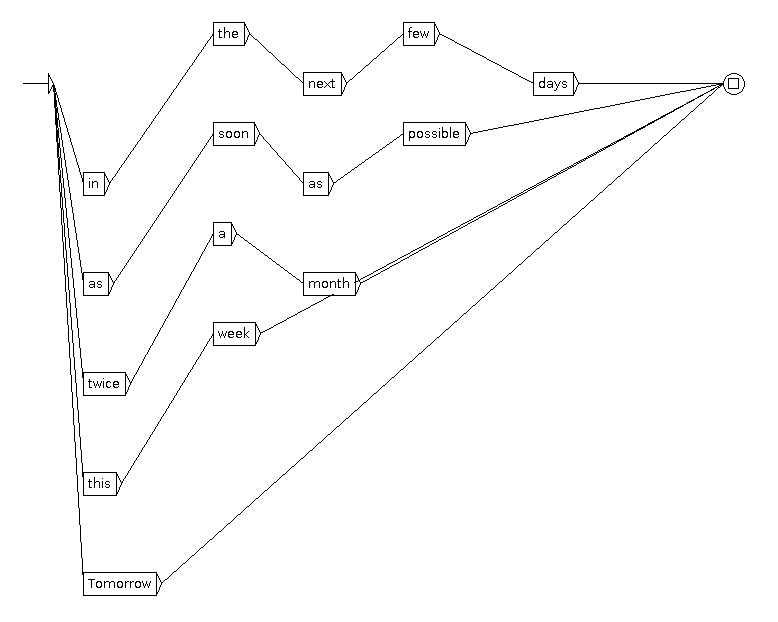
\includegraphics[width=8cm]{resources/img/fig8-5GRFnoBeautify.png}	
		\caption{Automate sans l'option "beautify"\label{fig8-5GRFnoBeautify}}
	\end{minipage}
	\hspace{0.1cm}
	\begin{minipage}[h!]{0.5\linewidth}
		\centering
		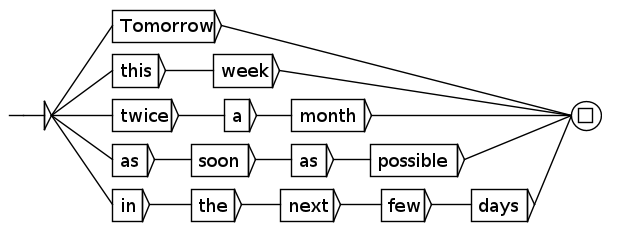
\includegraphics[width=8cm]{resources/img/fig8-6GRFBeautify.png}
		\caption{Automate avec l'option "beautify"\label{fig8-6GRFBeautify}}
	\end{minipage}
	\hspace{0.1cm}
\end{figure}
\pagebreak

%%%%%%%%%%%%%%%%%%%%%%%%%%%%%%%%%%%%%%%%%%%%%%%%%%%%%%%%%%%%%%%%%%%%%%%%%%%

\section{Recherche par approximation}
\label{approximation}

Lorsque vous effectuez un "Locate" sur un texte en utilisant un graphe produit avec le programme
\verb+Seq2Grf+, vous trouverez uniquement des séquences présentes dans le corpus de séquences
original. Des séquences proches de celles du corpus original peuvent être présentes dans le texte et
être ignorées parce qu'elles ne figurent pas dans ce corpus. Ces séquences devraient être incluses
dans l'automate de séquences. Afin d'inclure ces séquences, vous devez appliquer les trois sortes de
jokers et produire ainsi un graphe qui reconnaît toutes les  séquences du corpus, et les nouvelles séquences 
. Chaque joker, permet d'appliquer une opération pour générer de nouvelles séquences.
\begin{itemize}
	\item insertion : pour chaque séquence, ajouter à l'automate toutes les séquences où
	\verb+<TOKEN>+ a été inséré entre deux mots de la séquence originale.
	\item remplacement : pour chaque séquence, ajouter à l'automate toutes les séquences où $i$
		tokens ont été remplacés par \verb+<TOKEN>+
	\item suppression: pour chaque séquence, ajouter à l'automate toutes les séquences où un
		token a été supprimé
\end{itemize}
Chacune de ces opérations peut être appliquée plusieurs fois aux séquences originales. L'application
de cette grammaire à un texte permet d'introduire des approximations dans la recherche des séquences
du texte.

Si les jokers sont utilisés, les graphes produits suivent les règles suivantes :
\begin{itemize}
	\item les séquences originales et les séquences dérivées sont incluses dans l'automate,
	\item aucune séquence vide, ni une séquence composée uniquement de jokers ne seront ajoutées
		à ce graphe (de telles séquences peuvent être produites par des suppressions ou des
			remplacements sur des séquences courtes)
	\item pas d'insertion de jokers au début ou à la fin d'une séquence
	\item chaque token d'une séquence y compris le premier et le dernier peuvent être remplacés
		par un joker
\end{itemize}
Les graphes produits en utilisant des jokers contiennent de nombreuses séquences erronées et doivent
être confrontées avec le corpus au moyen de \verb+Locate+ pour ne garder que les séquences
pertinentes. Ces séquences peuvent être utilisées pour produire un nouveau graphe, que vous voudrez
peut-être garder.
\bigskip

Le graphe de la figure ~\ref{fig8-7GRF1replace} a été produit avec remplacement de 1 token et avec
l'option "beautifying" activée. (cf. figure ~\ref{fig8-2CorpusSNT})
\begin{figure}[h!]
	\begin{center}
		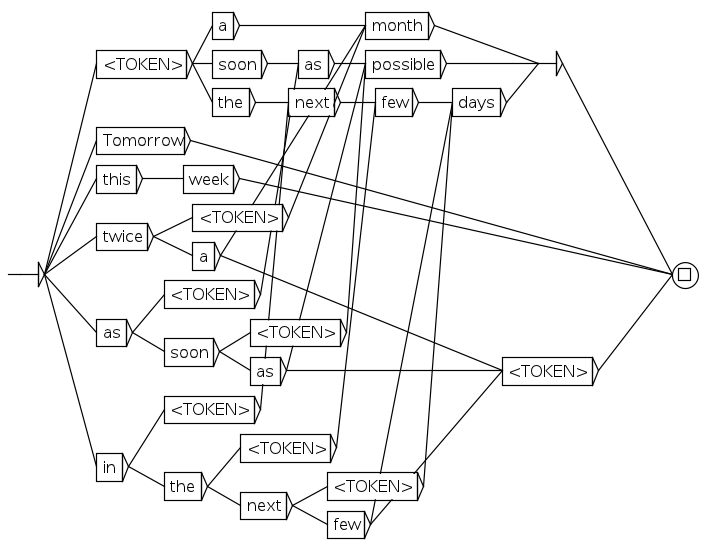
\includegraphics[width=8cm]{resources/img/fig8-7GRF1replace.png}
		\caption{Automate avec un remplacement permis\label{fig8-7GRF1replace}}
	\end{center}
\end{figure}
